\documentclass{article}
\usepackage[italian]{babel}
\usepackage{csquotes}
\usepackage[T1]{fontenc}
\usepackage{amsmath,amssymb,amsthm}
\usepackage{clrscode3e}

\usepackage{biblatex}
\addbibresource{./bibliography.bib}

\usepackage{enumerate}

\usepackage{epigraph}
\renewcommand{\epigraphrule}{0pt}
\renewcommand{\textflush}{flushepinormal}
\setlength{\epigraphwidth}{0.275\textwidth}
\renewenvironment{flushepinormal}{}{\vspace*{-\baselineskip}}

\usepackage{fontspec}
\usepackage{graphicx}
\usepackage{hyperref}
\usepackage{verbatim}

\graphicspath{ {./images/} }

\title{
  {
    \fontspec[ Path = fonts/ ]{Symbola}
    \symbol{"1F17C}\symbol{"1F435}\symbol{"1F17D}\symbol{"1F17A}ey
  } \large \\
  \small Relazione del progetto per l'insegnamento di Algoritmi e strutture di
  dati
}

\author{
  Gaia Clerici (\#971338),
  Stefano Volpe (\#969766)
}

\date{
	Universit\`a di Bologna \\
  \today
}

\begin{document}

\maketitle
\thispagestyle{empty}

\begin{figure}[h]
  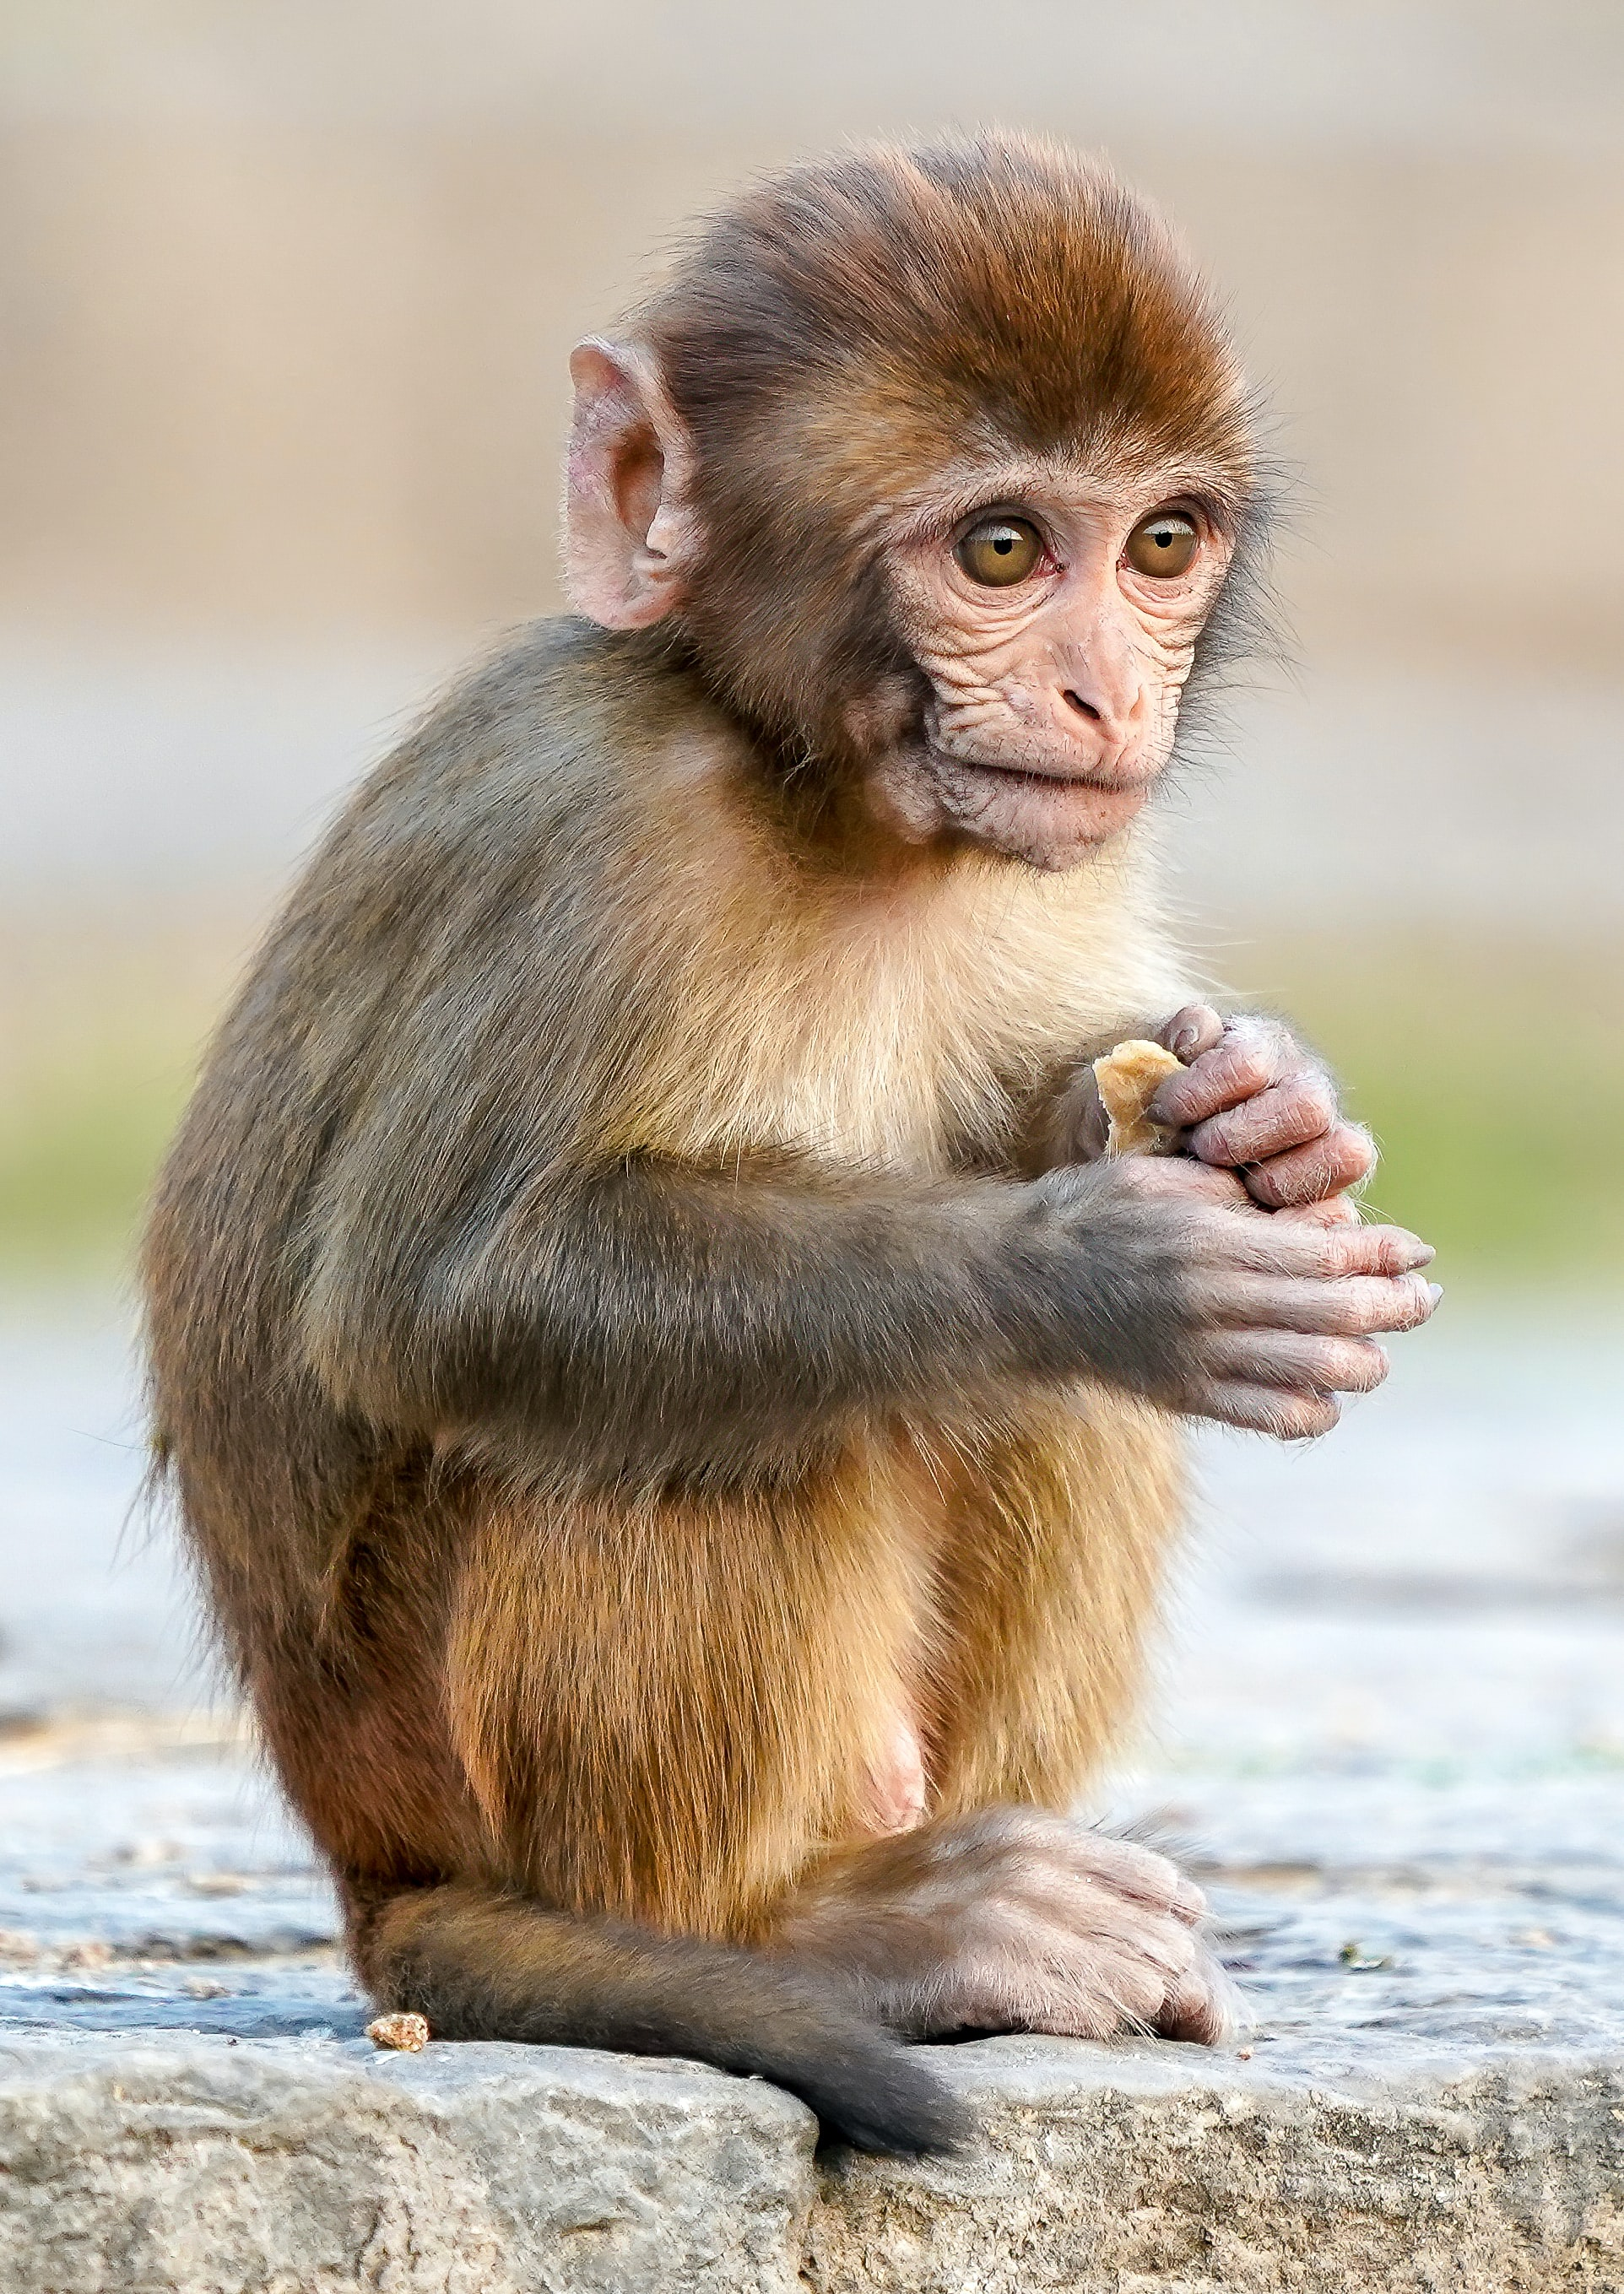
\includegraphics[width=0.75\textwidth]{monkey}
  \centering
  \caption{\href{https://unsplash.com/photos/daC7ji1EMHM}{una scimmia (foto di
  Bob Brewer)}}
\end{figure}

\pagebreak

\epigraph{Fa' la brava scimmietta.}{\textit{L'uomo con il cappello giallo}}

\tableofcontents

\pagebreak

\section{Specifiche}

\subsection{Il gioco: \emph{m,n,k-game}}

Il gioco \emph{m,n,k-game} è deterministico, a turni, a due giocatori, a somma
zero e con informazione perfetta. In una partita, i due agenti si alternano nel
marcare una cella vuota in una griglia di dimensione $m\times n$ con un simbolo
del proprio colore. Se un giocatore allinea in orizzontale, verticale o
diagonale almeno \emph{k} simboli, questi vince la partita e il suo avversario
la perde. Se non rimangono più celle vuote sulla griglia, la partita finisce
in pareggio.

\subsection{Il torneo: la classifica dei giocatori}

Ogni volta che, all'interno del torneo, un giocatore conclude una partita, egli
guadagna: 
\begin{itemize}
  \item 3 punti in caso di una vittoria come secondo giocatore, ma non a
    tavolino;
  \item 2 punti in caso di una vittoria come primo giocatore o a tavolino;
  \item 1 punto in caso di un pareggio;
  \item 0 punti in caso di una sconfitta.
\end{itemize}

\noindent
Le regole del torneo considerano una vittoria ``a tavolino'' quando l'avversario
non restituisce una mossa entro il tempo limite (approssimativo) di 10 secondi,
o comunque un mossa illegale (già occupata o esterna alla griglia). Non è dato
conoscere l'identità dell'avversario. Per ognuna delle seguenti configurazioni,
ciascun giocatore gioca esattamente quattro partite contro ogni altro
partecipante, di cui due come primo giocatore e due come secondo giocatore.

\begin{table}[h!]
\centering
\begin{tabular}{ | c | c | c | }
  \hline
  M & N & K \\
  \hline
  3 & 3 & 3 \\
  \hline
  4 & 3 & 3 \\
  \hline
  4 & 4 & 3 \\
  \hline
  4 & 4 & 4 \\
  \hline
  5 & 4 & 4 \\
  \hline
  5 & 5 & 4 \\
  \hline
  5 & 5 & 5 \\
  \hline
  6 & 4 & 4 \\
  \hline
  6 & 5 & 4 \\
  \hline
  6 & 6 & 4 \\
  \hline
  6 & 6 & 5 \\
  \hline
  6 & 6 & 6 \\
  \hline
  7 & 4 & 4 \\
  \hline
  7 & 5 & 4 \\
  \hline
  7 & 6 & 4 \\
  \hline
  7 & 7 & 4 \\
  \hline
  7 & 5 & 5 \\
  \hline
  7 & 6 & 5 \\
  \hline
  7 & 7 & 5 \\
  \hline
  7 & 7 & 6 \\
  \hline
  7 & 7 & 7 \\
  \hline
  8 & 8 & 4 \\
  \hline
  10 & 10 & 5 \\
  \hline
  50 & 50 & 10 \\
  \hline
  70 & 70 & 10 \\
  \hline
\end{tabular}
  \caption{configurazioni previste dal torneo.}
  \label{table:1}
\end{table}

\subsection{L'obiettivo: il giocatore}

Lo scopo del progetto è lo sviluppo di una intelligenza artificiale in Java
per il giocatore di \emph{m,n,k-game}. Se qualità della risposta e costo
temporale sono prioritari, lo stesso non vale per il costo in memoria, anche se
devono comunque essere evitati sprechi. Infine, a parità dei fattori di cui
sopra, la precedenza spetta alle strategie concettualmente più semplici.

\subsection{L'interfaccia: \texttt{mnkgame.MNKPlayer}}

L'interfaccia che l'intelligenza artificiale deve implementare è contenuta nel
pacchetto \verb!mnkgame!. Oltre a un metodo per la selezione della mossa
desiderata, ne viene concesso un altro invocato in fase di inizializzazione
prima di ogni partita.

\section{Analisi del problema}

\subsection{Il valore di gioco teorico}

Molte istanze del problema in questione si presentano come giochi a sé stanti,
talvolta arrichiti con limitazioni imposte dalle regole: ne sono esempi Tris,
Go-Moku e Renju. Per alcune configurazioni, il valore di gioco teorico è già
stato dimostrato. Van den Herik, Uiterwijk e van Rijswijck
\cite{VANDENHERIK2002277} hanno raccolto tali risultati dalla letteratura
precedente nella seguente tabella.

\begin{table}[h!]
  \centering
  \begin{tabular}{ | c | c | c | }
    \hline
    mnk-game (k=1,2) & Vittoria per il primo giocatore \\
    \hline
    333-game (Tris) & Pareggio \\
    \hline
    mn3-game ($m \geq 4, n \geq 3$) & Vittoria per il primo giocatore \\
    \hline
    m44-game ($m \leq 8$) & Pareggio \\
    \hline
    mn4-game ($m \leq 5,n \leq 5$) & Pareggio \\
    \hline
    mn4-game ($m \geq 6,n \geq 5$) & Vittoria per il primo giocatore \\
    \hline
    mn5-game ($m \leq 6,n \leq 6$) & Pareggio \\
    \hline
    15,15,5-game (Go-Moku) & Vittoria per il primo giocatore \\
    \hline
    mnk-game ($k \geq 8$) & Pareggio \\
    \hline
  \end{tabular}
    \caption{valori di gioco di \emph{m,n,k-game}}
    \label{table:2}
  \end{table}

Tramite l'argomento del ``furto di strategia'', usato per la prima volta da John
Nash nel 1949 \cite{at.UBO716493520180101}, si dimostra che nessuno dei valori
di gioco teorico non ancora aggiunto alla tabella è una vittoria per il secondo
giocatore.

\subsection{L'albero di gioco}

Van den Herik, Uiterwijk e van Rijswijck \cite{VANDENHERIK2002277} classificano
\emph{m,n,k-game} come di ``categoria 3'', ovvero con un'alta complessità dello
spazio degli stati e una bassa complessità dell'albero di gioco. Per poter
quantificare meglio il numero di stati effettivamente appartenenti al nostro
albero di gioco, faremo uso del numero di celle della griglia come indice della
dimensione dell'istanza del problema. Esso vale:

\begin{equation}
s = m \times n
\end{equation}

Cominciamo osservando che il numero di figli $f$ di un qualsiasi nodo non
terminale a profondità $p$ coincide con il numero di celle rimaste vuote, e
cioè:

\begin{equation}
  f(p) = s - p
\end{equation}

Se assumessimo che tutte le foglie dell'albero si trovassero a profondità $s$,
potremmo facilmente calcolare il numero di nodi $n$ a una data profondità $p$:

\begin{equation}
  n(p) = \frac{s!}{f(p)!}
\end{equation}

Quindi, sempre sotto questa ipotesi, il numero di nodi dell'albero sarebbe dato
da:

\begin{equation}
 \overline{n_{tot}} = \sum_{p = 0}^{s} n(p) = \sum_{p = 0}^{s} \frac{s!}{f(p)!} = s! \sum_{p = 0}^{s} \frac{1}{p!} = \Theta (s!)
\end{equation}

Una stima per difetto dell'effettivo numero di nodi è fornita dall'albero di
gioco le cui partite terminano tutte nel minor numero di mosse possibili.
Essendo ragionevole assumere

\begin{equation}
  m, n > 1 \wedge k \leq m, n
\end{equation}

si ha $2k - 1 < s$ e quindi:

\begin{equation}
  n_{tot} = \Omega ((2k - 1)!)
\end{equation}



\section{Strumenti}

\section{Scelte progettuali}

Oltre a \verb!MoNKey.java!, che implementa \verb!mnkgame.MNKPlayer!, e
\verb!Tester.java!, classe di collaudo del progetto, \verb!monkey! disponde di
tre sottopacchetti:
\begin{itemize}
  \item \verb!monkey.util! fornisce strutture dati e algoritmi di uso generale
    ma non presenti nella libreria standard Java;
  \item \verb!monkey.ai! definisce un'intelligenza artificale per un generico
    gioco a turni a due giocatori i cui stati siano istanze di un'unica classe
    implementante \verb!monkey.ai.State!;
  \item \verb!monkey.mnk! espone la rappresentazione di \emph{m,n,k-game}
    implementando \verb!monkey.ai.State!.
\end{itemize}

\subsection{\texttt{monkey.util}}

\begin{sloppypar}
Questo pacchetto sopperisce alle mancanze della libreria standard con i metodi
per il calcolo del minimo e del massimo fra due elementi, nonché con una mappa
implementata come tabella ad indirizzamento diretto
\cite{at.UBO708344820100101}. Da notare che, fatta eccezione per
l'inizializzazione della suddetta mappa (che ha un costo temporale lineare nella
sua capacità), tutti i metodi di questo pacchetto hanno costo costante.
\end{sloppypar}

\subsection{\texttt{monkey.ai}}

L'intelligenza artificiale progettata propone due diversi algoritmi per la
scelta della mossa: il primo effettua una ricerca all'interno dell'albero di
gioco, mentre il secondo un più veloce ma meno accurato confronto fra le mosse
al momento disponibili. Quest'ultimo è pensato per le configurazioni troppo
impegnative per il primo algoritmo. Spetta a \verb!MoNKey.java! decidere a quale
metodo fare affidamento basandosi su $s$.

\subsubsection{Ricerca nell'albero di gioco}

Nonostante Herik, Uiterwijk e Rijswijck \cite{VANDENHERIK2002277} raccomandino
per i giochi di ``categoria 3'' l'uso di metodi basati sulla conoscenza,
abbiamo optato per una scelta più tradizionalista: una sintesi di più varianti
della potatura alfa-beta, che si colloca invece nei metodi a forza bruta.

\begin{sloppypar}
In primo luogo, viste le imposizioni sul tempo di esecuzione, il nostro
algoritmo ha necessariamente bisogno di un limite di profondità $d$.
L'interfaccia delle due funzioni per una "classica" potatura alfa-beta
\cite{at.UBO029034619980101.200--202} risulta quindi essere:
\end{sloppypar}
\begin{itemize}
  \item $\proc{Max-Value}(s, \alpha, \beta, d)$: applica la ricerca
    al nodo che rappresenta lo stato $s$ assumendo che esso sia di massimo;
  \item $\proc{Min-Value}(s, \alpha, \beta, d)$: applica la ricerca
    al nodo che rappresenta lo stato $s$ assumendo che esso sia di minimo.
\end{itemize}
In entrambi i casi, $\alpha$ e $\beta$ fungono da parametri della potatura,
mentre $d$ è il limite di profondità imposto. La mutuale ricorsione di queste
due procedure è responsabile di un'esplorazione a profondità limitata
dell'albero; tale ricerca supporta il dietrofront
\cite{at.UBO029034619980101.108} (\emph{backtracking}) tramite le funzioni
$\proc{Result}(s, a)$ e $\proc{Revert}(s)$.
La loro implementazione non viene riportata in quanto piuttosto canonica,
eccezion fatta per ripetuti controlli sullo scadere del tempo di gioco e per
l'uso di una tabella delle trasposizioni \cite{CN020689428}. Tale tavola
\emph{hash} è a due livelli e fa uso dello schema di rimpiazzamento
$\proc{TwoBig1}$: Breuker, Uiterwijk e van den Herik
\cite{BREUKER-UITERWIJK-VANDENHERIK}
\cite{edsdbl.journals.icga.BreukerUH9619960101} ne hanno dimostrato la
superiorità rispetto a $\proc{Deep}$, $\proc{New}$, $\proc{Old}$, $\proc{Big1}$,
$\proc{BigAll}$ e $\proc{TwoDeep}$.

La variante della potatura alfa-beta scelta, che fa uso di $\proc{Max-Value}$ e
$\proc{Min-Value}$, è la ricerca del nodo migliore (\emph{best node search}, o
\emph{BNS}) di Rutko \cite{edseul.200009163084620110101}, che porta a
prestazioni migliori rispetto a tutte le varianti precedenti, vale a dire
$\proc{PVS}$, $\proc{Negascout}$, $\proc{NegaC*}$, $\proc{SSS*}$,
$\proc{Dual*}$, $\proc{MTD}(f)$. Il nostro algoritmo presenta varie differenze
rispetto alla versione originale:
\begin{itemize}
    \item il chiamante specifica il limite di profondità $d$ desiderato;
    \item il calcolo degli inizializzatori per $\alpha$ e $\beta$ viene delegato
      nelle linee \ref{li:initial-alpha} e \ref{li:initial-beta} allo stato
      corrente $s$, che può così effettuare considerazioni specifiche per il
      gioco in questione;
    \item proprio come per $\proc{Max-Value}$ e $\proc{Min-Value}$, gli unici
      sottoalberi ispezionati sono quelli considerati ``rilevanti'' da $s$ (vedi
      \ref{pattern-search});
    \begin{sloppypar}
    \item se più sottoalberi superano una prova, $\id{best-node}$ ne memorizza
      sempre il primo. Questo permette di approfittare del fatto che
      l'interfaccia \verb!monkey.ai.State! promette un'iterazione sulle azioni
      rilevanti in ordine decrescente di aspettative;
    \end{sloppypar}
    \item l'algoritmo originale, ispirandosi a $\id{Negamax}$, sostituiva alla
      chiamata a $\proc{Min-Value}$ della linea \ref{li:min-value} una a
      $\proc{Max-Value}$ con argomenti e valore resituito negati di segno. La
      nostra accezione di ``giochi a somma zero'' designa però i giochi a somma
      costante, per i quali tale espediente non è utilizzabile nel caso
      generale: evitarlo ci permette di fare uso di funzioni di valutazione
      degli stati asimmetriche rispetto ai due giocatori;
    \item la nostra esplorazione dell'albero, come già detto, supporta il
      dietrofront (linea \ref{li:backtracking}).
\end{itemize}

\begin{codebox}
  \Procname{$\proc{Best-Node-Search}(s, d)$}
  \li  $\alpha \gets \proc{Initial-Alpha}(s)$ \label{li:initial-alpha}
  \li  $\beta \gets \proc{Initial-Beta}(s)$ \label{li:initial-beta}
  \li  $\id{subtree-count} \gets \proc{Count-Relevant-Children}(s)$
  \li  \Repeat
  \li    $\id{best-node} \gets \const{nil}$
  \li    $\id{test} \gets \proc{Next-Guess}(\alpha, \beta, \id{subtree-count})$
  \li    $\id{better-count} \gets 0$
  \li    \For ogni azione rilevante $a$ di $s$
  \li      \Do
             \If $\proc{Min-Value}(\proc{Result}(s, a), test - 1, test, d) \geq
             test)$ \label{li:min-value}
  \li          \Then
                 $\id{better-count} \gets \id{better-count} + 1$
  \li            \If $\id{best-node} \isequal \const{nil}$
  \li              \Then
                     $\id{best-node} \gets a$
                   \End
               \End
  \li        $\proc{Revert}(s)$ \label{li:backtracking}
           \End
  \li    \If $\id{better-count} \isequal 0$
  \li      \Then $\beta \gets \id{test}$
  \li    \ElseIf $\id{better-count} > 1$
  \li      \Then
             $\id{subtree-count} \gets \id{better-count}$
  \li        $\alpha \gets \id{test}$
           \End
  \li  \Until $(\beta - \alpha < 2 \mbox{ or } \id{better-count} \isequal 1)
       \mbox{ and } \id{better-count} \neq 0$
  \li  \Return $\id{best-node}$
\end{codebox}

\begin{codebox}
  \Procname{$\proc{Next-Guess}(\alpha, \beta, \id{subtree-count})$}
  \li  \Return $\alpha + \frac{(\beta - \alpha) (\id{subtree-count} - 1)}
       {\id{subtree-count}}$
\end{codebox}

Il limite di profondità $d$ è stabililto da una ricerca ad approfondimento
iterativo. Rispetto alla versione proposta da Russel e Norvig
\cite{at.UBO029034619980101.109--111}, la nostra differisce sotto alcuni aspetti
e ne espande altri che erano stati originariamente solo accennati dagli autori:
\begin{itemize}
    \item l'intervallo dei possibili limiti di profondità ha un estremo
      superiore finito la cui scelta può dipendere da considerazioni specifiche
      su un gioco e uno stato particolari (linea \ref{li:max-limit});
    \item qualora una chiamata a $\proc{Best-Node-Search}$ segnali lo scadere
      del tempo, viene restituita la mossa calcolata con la più profonda ricerca
      completata;
    \item La linea \ref{li:setup-backup} memorizza una copia dello stato di
      gioco di partenza. In questo modo, in caso di terminazione urgente dovuta
      allo scadere del tempo di gioco, è possibile ripristinare alla linea
      \ref{li:restore-backup} tale copia con costo temporale costante. Nessuna
      pila di chiamate $\proc{Best-Node-Search}$, $\proc{Max-Value}$ e
      $\proc{Min-Value}$ dovrà così affannarsi a invertire l'effetto di più
      mosse di gioco una per una.
\end{itemize}
\begin{sloppypar}
Lo pseudocodice che segue impiega un semplice sistema di gestione delle
eccezioni alla linea \ref{li:try}. Questo ha permesso di codificare
$\proc{Best-Node-Search}$ facendo affidamento al principio dell'``acchiappa e
rilascia'', e ignorando così la gestione delle scadenze temporali, che viene
delegata a ipotetiche implementazioni di $\proc{Max-Value}$ e
$\proc{Min-Value}$. Ovviamente, è comunque possibile (e fruttuoso a livello di
prestazioni) fare affidamento a valori restituiti dalle varie funzioni che
segnalino questo tipo di occorrenze.
\end{sloppypar}

\begin{codebox}
  \Procname{$\proc{Iterative-Deepening-Search}(s)$}
  \li  $\id{backup-state} \gets \proc{copy}(s)$ \label{li:setup-backup}
  \li  $\id{max-limit} \gets \proc{Overestimated-Height}(s)$
       \label{li:max-limit}
  \li  $\id{res} \gets \const{nil}$
  \li  \For $d \gets 0$ \To $\id{max-limit}$
  \li    \Do
           \kw{try} \label{li:try}
  \li        \Do
               $\id{res} \gets \proc{Best-Node-Search}(d)$
             \End
  \li      \kw{catch} $\const{timeout-exception}$
  \li        \Do
               $s \gets \id{backup-state}$ \label{li:restore-backup}
  \li          \If $\id{res} \neq \const{nil}$
  \li            \Then
                   \Return $\id{res}$
                 \End
  \li          \Comment fallback action
  \li          \Return $\proc{First-Relevant-Action}(s)$
             \End
         \End
  \li  \Return $\id{res}$
\end{codebox}

\subsubsection{Confronto fra mosse}

Questa secondo modo di individuare una mossa promettente ne estrae una in modo
pseudorandomico fra quelle che, applicate allo stato attuale, massimizzano la
funzione di valutazione. Anche questo algoritmo supporta il dietrofront e si
limita ad analizzare le azioni considerate ``rilevanti''.

\begin{codebox}
  \Procname{$\proc{Immediate-Search}(s)$}
  \li  $\id{best-moves} \gets$
       {\fontspec[ Path = fonts/ ]{Symbola}\emph{\symbol{"2205}}}
  \li  $\id{max-eval} \gets \const{nil}$
  \li \For ogni azione rilevante $a$ di $s$
  \li   \Do
          $\id{current-eval} \gets \proc{Eval}(\proc{Result}(s, a))$
  \li     $\proc{Revert}(s)$
  \li     \If $\id{max-eval} \isequal \const{nil}$
  \li       \Then
              $\id{max-eval} \gets \id{current-eval}$
  \li         $\id{best-moves} \gets \id{best-moves} \cup \{ a \}$
  \li     \ElseIf $\id{current-eval} \geq \id{max-eval}$
  \li       \Then
              \If $\id{current-eval} > \id{max-eval}$
  \li           \Then
                  $\id{max-eval} \gets \id{current-eval}$
  \li             $\id{best-moves} \gets$
                  {\fontspec[ Path = fonts/ ]{Symbola}\emph{\symbol{"2205}}}
                \End
  \li         $\id{best-moves} \gets \id{best-moves} \cup \{ a \}$
          \End
        \End
  \li  \Return \proc{Random}(\id{best-moves})
\end{codebox}

\subsection{\texttt{monkey.mnk}}

\subsubsection{Stato iniziale}

\subsubsection{Inizializzatori per $\alpha$ e $\beta$}

\subsubsection{Azioni} \label{pattern-search}

\subsubsection{Modello di transizione}

\subsubsection{Funzione di valutazione}

\subsubsection{Funzione di \emph{hashing}}

\section{Conclusioni}

\section{Ricerche future}

\pagebreak

\begin{sloppypar}
\printbibliography[
  heading=bibintoc
]
\end{sloppypar}

\end{document}
